\chapter{System Design}

\section{Introduction}
The system design phase defines the architecture, components, and data flow of the **Donation Platform with Payment Gateway**. This chapter provides a detailed **high-level and low-level design**, covering **architectural diagrams, database schema, and module interactions**.

\section{System Architecture}
The system follows a **MERN stack (MongoDB, Express.js, React.js, Node.js) architecture**, ensuring scalability, modularity, and security.

\subsection{Architectural Design}
The system is structured into three main layers:
\begin{itemize}
    \item \textbf{Presentation Layer:} The **React.js frontend** provides an interactive UI for users.
    \item \textbf{Business Logic Layer:} The **Node.js backend (Express.js)** processes user requests and handles API calls.
    \item \textbf{Data Layer:} The **MongoDB database** stores user profiles, donation records, and campaign details.
\end{itemize}

\section{Database Design}
The database is designed using **MongoDB**, which stores data in a **NoSQL document format**. The key collections and their attributes are as follows:

\subsection{User Collection (Admin, NGO, Company, Donor)}
\begin{verbatim}
{
    _id: ObjectId("67d7a2a13da1bcc7eb4cb838"),
    full_name: "NGO",
    email: "ngo@gmail.com",
    phone: "1100543410",
    password: "$2b$10$ax/267EibhZNJD2pKZJgD.huNlrouwvs/x7dPKIsS",
    role: "NGO", // Admin / NGO / Company / Donor
    is_verified: false,
    is_active: true,
    approval_status: "Pending",
    created_at: ISODate("2025-03-17T04:18:41.544Z"),
    updated_at: ISODate("2025-03-17T04:18:41.544Z"),
    __v: 0
}

\end{verbatim}
\begin{figure}[h]
    \centering
    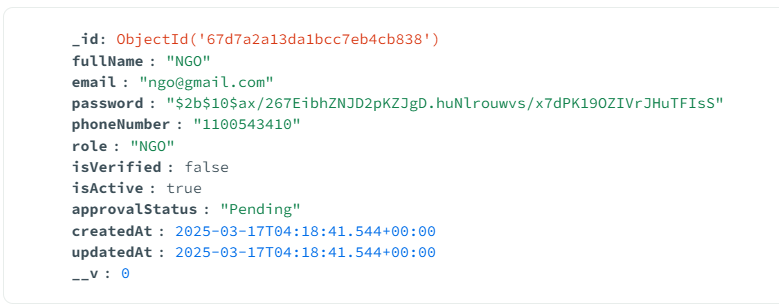
\includegraphics[width=0.8\textwidth]{images/user collection.png} % Adjust width as needed
    \caption{User Collection}
    \label{fig: User Collection}
\end{figure}

\subsection{NGO Collection}
\begin{verbatim}
{
    _id: ObjectId("67d7a2a13da1bcc7eb4cb83a"),
    user_id: ObjectId("67d7a2a13da1bcc7eb4cb838"),
    ngo_name: "NGO",
    email: "ngo@gmail.com",
    contact_number: "1100543410",
    registration_number: null,
    registered_year: null,
    address: null,
    website: null,
    
    authorized_person: {
        pan_number: null,
        tan_number: null,
        gst_number: null
    },

    number_of_employees: null,
    ngo_type: null,
    is_80G_certified: false,
    is_12A_certified: false,

    bank_details: {},
    logo: null,
    is_active: true,
    
    created_at: ISODate("2025-03-17T04:18:41.553Z"),
    updated_at: ISODate("2025-03-17T04:18:41.553Z"),
    __v: 0
}
\end{verbatim}
\begin{figure}[h]
    \centering
    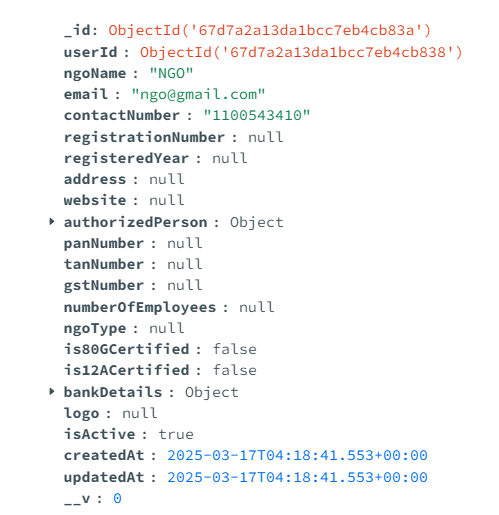
\includegraphics[width=0.5\textwidth]{images/NGO_Collection.png}
    \caption{NGO Collection}
    \label{fig:ngo_collection}
\end{figure}

\subsection{Campaign Collection}
\begin{verbatim}
{
    _id: ObjectId,
    title: String,
    description: String,
    goal_amount: Number,
    raised_amount: Number,
    start_date: Date,
    end_date: Date,
    created_by: ObjectId (Reference to NGO),
    donations: [ObjectId] (Reference to Donations)
}
\end{verbatim}

\subsection{Donation Collection}
\begin{verbatim}
{
    _id: ObjectId,
    donor_id: ObjectId (Reference to User),
    campaign_id: ObjectId (Reference to Campaign),
    amount: Number,
    payment_status: String (Success / Pending / Failed),
    transaction_id: String,
    created_at: Timestamp
}
\end{verbatim}

\section{Module Design}
The system consists of several core modules:

\subsection{User Authentication Module}
\begin{itemize}
    \item **Sign-up/Login:** Secure JWT-based authentication.
    \item **Password Encryption:** Uses **bcrypt** for secure password storage.
    \item **Role-Based Access Control (RBAC):** Defines user privileges.
\end{itemize}

\subsection{Campaign Management Module}
\begin{itemize}
    \item NGOs can **create, update, delete** campaigns.
    \item Admins can **approve or reject** campaigns.
    \item Donors can **browse and contribute** to campaigns.
\end{itemize}

\subsection{Donation Processing Module}
\begin{itemize}
    \item Integrates **Cashfree Payment Gateway** for seamless transactions.
    \item Supports multiple payment methods: **UPI, Net Banking, Debit/Credit Cards**.
    \item Generates **donation receipts** for tax exemption.
\end{itemize}

\subsection{Admin Dashboard Module}
\begin{itemize}
    \item View and manage **users, NGOs, and campaigns**.
    \item Access **donation reports and analytics**.
    \item Approve or disable NGOs and campaigns.
\end{itemize}

\subsection{Reports and Analytics Module}
\begin{itemize}
    \item Generate **donation reports** for NGOs, companies, and donors.
    \item Display **campaign performance statistics**.
    \item Track **donation trends over time**.
\end{itemize}

\section{User Interface Design}
The frontend is built using **React.js**, ensuring a user-friendly experience. Key UI elements include:

\subsection{Login and Registration Page}
\begin{itemize}
    \item Users can sign up and log in with **secure authentication**.
    \item Role-based redirection after login.
\end{itemize}

\subsection{Campaign Dashboard}
\begin{itemize}
    \item NGOs can create and track campaigns.
    \item Donors can browse and contribute to campaigns.
\end{itemize}

\subsection{Donation Page}
\begin{itemize}
    \item Displays campaign details and available donation methods.
    \item Secure payment processing through **Cashfree**.
\end{itemize}

\subsection{Admin Panel}
\begin{itemize}
    \item View and manage all users, campaigns, and donations.
    \item Access **real-time donation reports**.
\end{itemize}
